% Options for packages loaded elsewhere
\PassOptionsToPackage{unicode}{hyperref}
\PassOptionsToPackage{hyphens}{url}
\documentclass[
]{article}
\usepackage{xcolor}
\usepackage[margin=1in]{geometry}
\usepackage{amsmath,amssymb}
\setcounter{secnumdepth}{-\maxdimen} % remove section numbering
\usepackage{iftex}
\ifPDFTeX
  \usepackage[T1]{fontenc}
  \usepackage[utf8]{inputenc}
  \usepackage{textcomp} % provide euro and other symbols
\else % if luatex or xetex
  \usepackage{unicode-math} % this also loads fontspec
  \defaultfontfeatures{Scale=MatchLowercase}
  \defaultfontfeatures[\rmfamily]{Ligatures=TeX,Scale=1}
\fi
\usepackage{lmodern}
\ifPDFTeX\else
  % xetex/luatex font selection
\fi
% Use upquote if available, for straight quotes in verbatim environments
\IfFileExists{upquote.sty}{\usepackage{upquote}}{}
\IfFileExists{microtype.sty}{% use microtype if available
  \usepackage[]{microtype}
  \UseMicrotypeSet[protrusion]{basicmath} % disable protrusion for tt fonts
}{}
\makeatletter
\@ifundefined{KOMAClassName}{% if non-KOMA class
  \IfFileExists{parskip.sty}{%
    \usepackage{parskip}
  }{% else
    \setlength{\parindent}{0pt}
    \setlength{\parskip}{6pt plus 2pt minus 1pt}}
}{% if KOMA class
  \KOMAoptions{parskip=half}}
\makeatother
\usepackage{longtable,booktabs,array}
\usepackage{calc} % for calculating minipage widths
% Correct order of tables after \paragraph or \subparagraph
\usepackage{etoolbox}
\makeatletter
\patchcmd\longtable{\par}{\if@noskipsec\mbox{}\fi\par}{}{}
\makeatother
% Allow footnotes in longtable head/foot
\IfFileExists{footnotehyper.sty}{\usepackage{footnotehyper}}{\usepackage{footnote}}
\makesavenoteenv{longtable}
\usepackage{graphicx}
\makeatletter
\newsavebox\pandoc@box
\newcommand*\pandocbounded[1]{% scales image to fit in text height/width
  \sbox\pandoc@box{#1}%
  \Gscale@div\@tempa{\textheight}{\dimexpr\ht\pandoc@box+\dp\pandoc@box\relax}%
  \Gscale@div\@tempb{\linewidth}{\wd\pandoc@box}%
  \ifdim\@tempb\p@<\@tempa\p@\let\@tempa\@tempb\fi% select the smaller of both
  \ifdim\@tempa\p@<\p@\scalebox{\@tempa}{\usebox\pandoc@box}%
  \else\usebox{\pandoc@box}%
  \fi%
}
% Set default figure placement to htbp
\def\fps@figure{htbp}
\makeatother
% definitions for citeproc citations
\NewDocumentCommand\citeproctext{}{}
\NewDocumentCommand\citeproc{mm}{%
  \begingroup\def\citeproctext{#2}\cite{#1}\endgroup}
\makeatletter
 % allow citations to break across lines
 \let\@cite@ofmt\@firstofone
 % avoid brackets around text for \cite:
 \def\@biblabel#1{}
 \def\@cite#1#2{{#1\if@tempswa , #2\fi}}
\makeatother
\newlength{\cslhangindent}
\setlength{\cslhangindent}{1.5em}
\newlength{\csllabelwidth}
\setlength{\csllabelwidth}{3em}
\newenvironment{CSLReferences}[2] % #1 hanging-indent, #2 entry-spacing
 {\begin{list}{}{%
  \setlength{\itemindent}{0pt}
  \setlength{\leftmargin}{0pt}
  \setlength{\parsep}{0pt}
  % turn on hanging indent if param 1 is 1
  \ifodd #1
   \setlength{\leftmargin}{\cslhangindent}
   \setlength{\itemindent}{-1\cslhangindent}
  \fi
  % set entry spacing
  \setlength{\itemsep}{#2\baselineskip}}}
 {\end{list}}
\usepackage{calc}
\newcommand{\CSLBlock}[1]{\hfill\break\parbox[t]{\linewidth}{\strut\ignorespaces#1\strut}}
\newcommand{\CSLLeftMargin}[1]{\parbox[t]{\csllabelwidth}{\strut#1\strut}}
\newcommand{\CSLRightInline}[1]{\parbox[t]{\linewidth - \csllabelwidth}{\strut#1\strut}}
\newcommand{\CSLIndent}[1]{\hspace{\cslhangindent}#1}
\setlength{\emergencystretch}{3em} % prevent overfull lines
\providecommand{\tightlist}{%
  \setlength{\itemsep}{0pt}\setlength{\parskip}{0pt}}
\usepackage{booktabs}
\usepackage{longtable}
\usepackage{array}
\usepackage{multirow}
\usepackage{float}
\usepackage{caption}
\captionsetup{font=small,labelfont=bf}
\renewcommand{\abstractname}{Resumo}
\renewcommand{\figurename}{Figura}
\renewcommand{\tablename}{Tabela}
\usepackage{booktabs}
\usepackage{longtable}
\usepackage{array}
\usepackage{multirow}
\usepackage{wrapfig}
\usepackage{float}
\usepackage{colortbl}
\usepackage{pdflscape}
\usepackage{tabu}
\usepackage{threeparttable}
\usepackage{threeparttablex}
\usepackage[normalem]{ulem}
\usepackage{makecell}
\usepackage{xcolor}
\usepackage{bookmark}
\IfFileExists{xurl.sty}{\usepackage{xurl}}{} % add URL line breaks if available
\urlstyle{same}
\hypersetup{
  pdftitle={Inferência Estatística Ainda É Minoritária em Seis Periódicos Brasileiros, 2005--2025},
  hidelinks,
  pdfcreator={LaTeX via pandoc}}

\title{Inferência Estatística Ainda É Minoritária em Seis Periódicos
Brasileiros, 2005--2025}
\author{}
\date{\vspace{-2.5em}18 de Julho de 2026}

\begin{document}
\maketitle
\begin{abstract}
Este artigo mensura a presença de pesquisa empírica, quantificação,
inferência estatística e estratégias explícitas de identificação causal
em periódicos brasileiros indexados no SciELO entre 2005 e 2025. O
universo elegível reúne 5.249 artigos de onze periódicos; 3.565 foram
classificados por modelos de linguagem a partir da leitura integral.
Seis periódicos estão integralmente cobertos e constituem o estrato
principal das comparações editoriais. Neles, apenas 551 de 1.281 artigos
quantitativos com informação válida para essa medida (43,0\%) apresentam
teste de hipótese, intervalo de confiança ou credibilidade, ou outra
quantificação formal de incerteza. Entre os cinco periódicos presentes
nos três períodos agregados, essa proporção permanece praticamente
estável: 46,1\% em 2005--2011, 44,2\% em 2012--2018 e 44,1\% em
2019--2025. A magnitude é próxima, mas não diretamente equivalente, à
parcela de abordagens baseadas em desenho causal entre artigos
quantitativos explicativos estimada por Torreblanca et al.~para o
Journal of Politics (45,4\%), a AJPS (47,0\%) e a APSR (56,8\%). Entre
os 846 artigos dos seis periódicos selecionados para examinar
identificação, apenas 49 (5,8\%) mencionam uma estratégia explícita. As
contagens registram presença, não qualidade de execução. Como a
classificação ainda requer validação humana, os resultados constituem um
diagnóstico preliminar.
\end{abstract}

\section{Introdução}\label{introduuxe7uxe3o}

O diagnóstico do ``calcanhar metodológico'' chamou atenção para as
limitações do treinamento em métodos na Ciência Política brasileira e
para seus efeitos sobre a acumulação de conhecimento
(\citeproc{ref-soares2005}{2005}). Barberia, Godoy e Barboza
(\citeproc{ref-barberia2014}{2014}) documentaram a expansão e a
distribuição desigual do ensino de métodos nos programas de
pós-graduação. Albuquerque, Mesquita e Brito
(\citeproc{ref-albuquerque2022}{2022}) examinaram a formação
metodológica em Relações Internacionais e áreas afins, enquanto
Figueiredo Filho et al. (\citeproc{ref-figueiredo2019}{2019}) defenderam
transparência e reprodutibilidade como condições para a avaliação
coletiva da pesquisa. Esses trabalhos tratam principalmente de formação
e normas de pesquisa. Este artigo observa o produto publicado: a
presença de evidência empírica, quantificação, inferência estatística e
estratégias explícitas de identificação causal.

O artigo pergunta como essas práticas se distribuem entre periódicos
brasileiros indexados no SciELO, entre 2005 e 2025. A mensuração
preserva o pluralismo metodológico da área. Estudos qualitativos,
históricos, interpretativos e normativos não precisam adotar um formato
único nem recorrer a estratégias causais. A comparação separa dimensões
que frequentemente são confundidas: um artigo pode ser empírico sem ser
quantitativo, quantitativo sem realizar inferência estatística e
explicativo sem mobilizar uma estratégia explícita de identificação
causal.

Torreblanca et al. (\citeproc{ref-torreblanca2026}{2026}) oferecem a
referência internacional para distinguir o corpus total, os artigos
empíricos, os trabalhos quantitativos, os estudos com afirmações causais
ou explicativas e aqueles que mencionam estratégias explícitas de
identificação. Partimos dessas distinções conceituais, mas adaptamos o
protocolo ao corpus brasileiro; não reproduzimos integralmente seu
classificador nem seus denominadores. Esperamos encontrar diferenças
entre periódicos e períodos, além de distância entre a presença de
afirmações causais ou explicativas e a menção a estratégias de
identificação. As comparações são descritivas: o desenho não identifica
por que periódicos ou períodos diferem.

Essa separação permite tratar a inferência estatística como resultado
substantivo, e não como sinônimo de quantificação. Estatísticas
descritivas resumem os casos observados; testes de hipótese, intervalos
e procedimentos equivalentes quantificam a incerteza de uma
generalização. Eles tampouco bastam para identificar efeitos causais.
Portanto, empiria, quantificação, inferência estatística e identificação
causal formam dimensões relacionadas, mas não degraus intercambiáveis de
uma mesma escala.

O universo elegível contém 5.249 artigos de onze periódicos. A
classificação por leitura integral cobre 3.565, ou 67,9\% do total. Seis
periódicos estão integralmente classificados e somam 2.321 artigos; as
comparações editoriais principais restringem-se a esse estrato. Neles,
551 de 1.281 artigos quantitativos com rótulo observado apresentam
inferência estatística (43,0\%). Entre os 846 artigos selecionados para
examinar identificação, 49 mencionam alguma estratégia explícita,
equivalentes a 5,8\%.

A contribuição é uma mensuração comparável de quatro dimensões da
prática publicada e um diagnóstico preliminar de sua heterogeneidade
editorial e temporal. A classificação automatizada ainda requer
validação humana, e sua configuração variou entre lotes; por isso, as
tendências são exploratórias e os resultados não representam o conjunto
da produção nacional. O artigo registra a presença declarada de métodos
e procedimentos, sem avaliar sua qualidade de execução.

\section{Dados}\label{dados}

Analiso artigos publicados entre 2005 e 2025 em onze periódicos
indexados no SciELO: \texttt{Brazilian\ Political\ Science\ Review},
\texttt{Opinião\ Pública},
\texttt{Revista\ Brasileira\ de\ Ciência\ Política},
\texttt{Revista\ de\ Sociologia\ e\ Política}, \texttt{Dados},
\texttt{Lua\ Nova}, \texttt{Novos\ Estudos\ CEBRAP},
\texttt{Revista\ Brasileira\ de\ Ciências\ Sociais},
\texttt{Contexto\ Internacional},
\texttt{Revista\ Brasileira\ de\ Política\ Internacional} e
\texttt{Cadernos\ Gestão\ Pública\ e\ Cidadania}. Juntos, esses
periódicos somam 5.249 artigos elegíveis no período.

Quatro periódicos mapeados no levantamento inicial não entram na análise
principal: \texttt{Brazilian\ Journal\ of\ Political\ Economy},
\texttt{Civitas\ -\ Revista\ de\ Ciências\ Sociais},
\texttt{Revista\ de\ Administração\ Pública} e
\texttt{Sur.\ Revista\ Internacional\ de\ Direitos\ Humanos}. As
exclusões foram definidas antes desta atualização para delimitar um
núcleo de Ciência Política, Relações Internacionais, gestão pública e
Ciências Sociais políticas. Como essa fronteira é contestável, os
critérios e as decisões são preservados no material de replicação. A
Tabela 1 apresenta o número de artigos elegíveis e classificados por
periódico e período.

Os textos integrais foram recuperados do SciELO em junho de 2026, e a
base analítica desta versão foi atualizada em 18 de julho de 2026. O
material de replicação preserva as fontes, as datas de acesso, as
decisões de exclusão e as verificações de integridade dos arquivos.

Esta versão usa 3.565 artigos já classificados, equivalentes a 67,9\% do
universo elegível. A cobertura é desigual.
\texttt{Brazilian\ Political\ Science\ Review},
\texttt{Cadernos\ Gestão\ Pública\ e\ Cidadania},
\texttt{Contexto\ Internacional}, \texttt{Dados},
\texttt{Opinião\ Pública} e
\texttt{Revista\ Brasileira\ de\ Ciência\ Política} estão integralmente
classificados e somam 2.321 artigos. Os outros cinco periódicos têm
cobertura parcial. Assim, o paper separa a cobertura integral dos
artigos de seis periódicos --- cujos rótulos automatizados ainda exigem
validação --- do retrato provisório formado por todos os artigos já
classificados.

\begin{longtable}[]{@{}
  >{\raggedright\arraybackslash}p{(\linewidth - 12\tabcolsep) * \real{0.2840}}
  >{\raggedright\arraybackslash}p{(\linewidth - 12\tabcolsep) * \real{0.1235}}
  >{\raggedright\arraybackslash}p{(\linewidth - 12\tabcolsep) * \real{0.1728}}
  >{\raggedright\arraybackslash}p{(\linewidth - 12\tabcolsep) * \real{0.1235}}
  >{\raggedright\arraybackslash}p{(\linewidth - 12\tabcolsep) * \real{0.0988}}
  >{\raggedright\arraybackslash}p{(\linewidth - 12\tabcolsep) * \real{0.0988}}
  >{\raggedright\arraybackslash}p{(\linewidth - 12\tabcolsep) * \real{0.0988}}@{}}
\caption{Artigos elegíveis e classificados por periódico e período. Nas
colunas de período, classificados/elegíveis.}\tabularnewline
\toprule\noalign{}
\begin{minipage}[b]{\linewidth}\raggedright
Periódico
\end{minipage} & \begin{minipage}[b]{\linewidth}\raggedright
Elegíveis
\end{minipage} & \begin{minipage}[b]{\linewidth}\raggedright
Classificados
\end{minipage} & \begin{minipage}[b]{\linewidth}\raggedright
Cobertura
\end{minipage} & \begin{minipage}[b]{\linewidth}\raggedright
2005-11
\end{minipage} & \begin{minipage}[b]{\linewidth}\raggedright
2012-18
\end{minipage} & \begin{minipage}[b]{\linewidth}\raggedright
2019-25
\end{minipage} \\
\midrule\noalign{}
\endfirsthead
\toprule\noalign{}
\begin{minipage}[b]{\linewidth}\raggedright
Periódico
\end{minipage} & \begin{minipage}[b]{\linewidth}\raggedright
Elegíveis
\end{minipage} & \begin{minipage}[b]{\linewidth}\raggedright
Classificados
\end{minipage} & \begin{minipage}[b]{\linewidth}\raggedright
Cobertura
\end{minipage} & \begin{minipage}[b]{\linewidth}\raggedright
2005-11
\end{minipage} & \begin{minipage}[b]{\linewidth}\raggedright
2012-18
\end{minipage} & \begin{minipage}[b]{\linewidth}\raggedright
2019-25
\end{minipage} \\
\midrule\noalign{}
\endhead
\bottomrule\noalign{}
\endlastfoot
CGPC & 120 & 120 & 100,0\% & 0/0 & 0/0 & 120/120 \\
BPSR & 268 & 268 & 100,0\% & 46/46 & 108/108 & 114/114 \\
Opinião Pública & 464 & 464 & 100,0\% & 117/117 & 163/163 & 184/184 \\
RBCP & 391 & 391 & 100,0\% & 29/29 & 194/194 & 168/168 \\
RSP & 638 & 406 & 63,6\% & 254/254 & 149/224 & 3/160 \\
Dados & 622 & 622 & 100,0\% & 181/181 & 212/212 & 229/229 \\
Lua Nova & 511 & 100 & 19,6\% & 100/141 & 0/188 & 0/182 \\
Novos Estudos CEBRAP & 581 & 132 & 22,7\% & 132/235 & 0/180 & 0/166 \\
RBCS & 708 & 300 & 42,4\% & 222/222 & 78/237 & 0/249 \\
Contexto Internacional & 456 & 456 & 100,0\% & 102/102 & 170/170 &
184/184 \\
RBPI & 490 & 306 & 62,4\% & 155/155 & 148/168 & 3/167 \\
\end{longtable}

\section{Estratégia Empírica}\label{estratuxe9gia-empuxedrica}

A estratégia empírica é uma estratégia de mensuração, não uma estratégia
de identificação causal do próprio paper. O objetivo é descrever como os
artigos se distribuem em dimensões metodológicas observáveis: presença
de evidência empírica, tipo de evidência, componente quantitativo,
inferência estatística, afirmação causal ou explicativa e menção a
estratégias explícitas de identificação causal. Os agregados dos 3.565
artigos classificados descrevem cobertura parcial. As comparações entre
periódicos usam apenas os seis periódicos completos; as comparações
temporais usam os cinco periódicos completos que publicaram nos três
períodos, com o mesmo peso para cada periódico.

O mapa de denominadores deve ser lido com cuidado. Algumas etapas são
aninhadas: a frequência das estratégias de identificação é calculada
dentro do subconjunto em que a identificação é metodologicamente
relevante. Outras dimensões são cruzadas: afirmações causais ou
explicativas podem aparecer em artigos qualitativos, quantitativos ou
mistos. Por isso, a Figura 1 apresenta denominadores e dimensões da
classificação disponível, e não uma sequência estritamente aninhada em
todos os degraus.

\begin{figure}
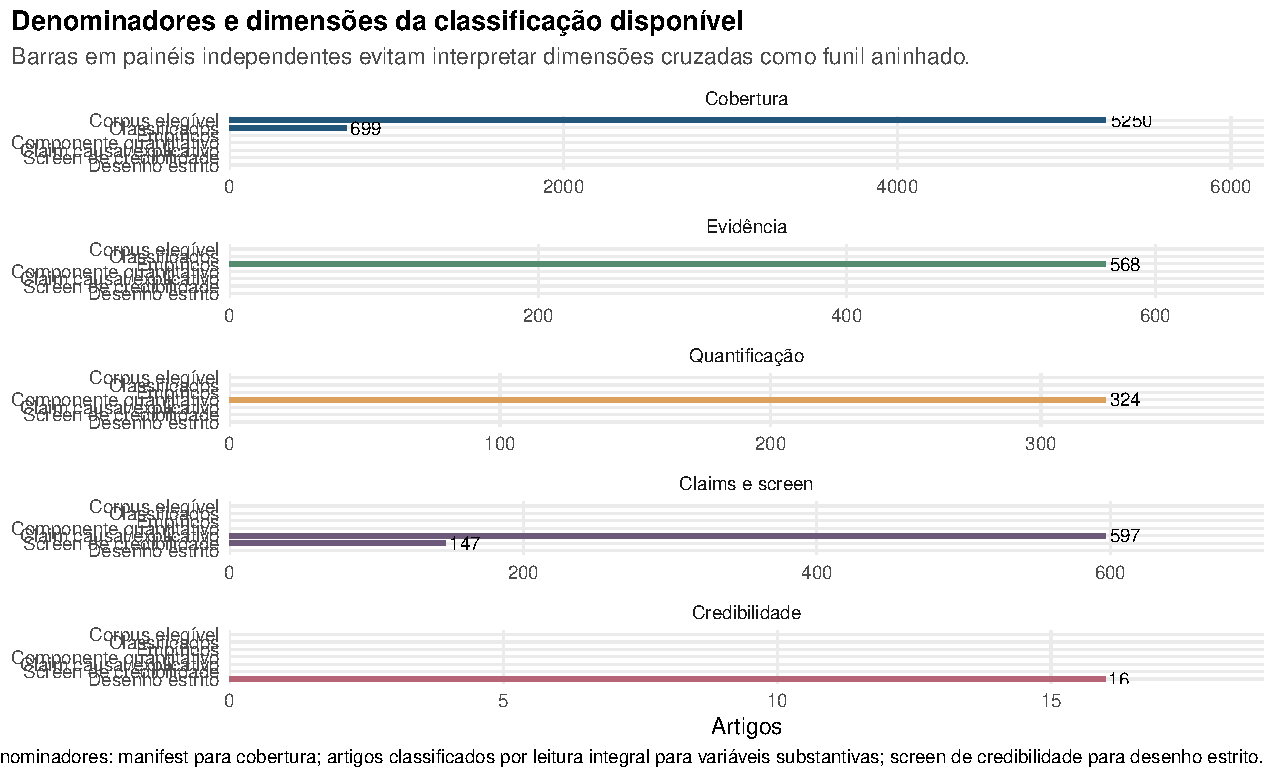
\includegraphics[width=0.95\linewidth]{../output/figures/paper/figure_1_corpus_funnel} \caption{Cobertura do corpus e incidência de práticas metodológicas. A cobertura usa os 5.249 artigos elegíveis; as demais linhas descrevem os 3.565 artigos classificados, com numerador e denominador indicados junto a cada ponto.}\label{fig:figura-1}
\end{figure}

O classificador registra primeiro se o artigo é empírico e que tipo de
evidência mobiliza: qualitativa, quantitativa, mista ou ausente. Em
seguida, distingue artigos com análise quantitativa, inferência
estatística e afirmações causais ou explicativas. Para examinar a camada
associada à identificação causal, o protocolo seleciona artigos por um
de dois caminhos: combinação de afirmação causal ou explicativa com
evidência empírica pertinente; ou emprego de modelagem quantitativa que
exige examinar como as inferências são sustentadas. Esse subconjunto não
equivale ao conjunto de estudos causais. Ele define apenas os artigos
nos quais procuramos, na etapa seguinte, menções a estratégias
explícitas de identificação.

Um artigo é classificado como contendo inferência estatística quando
reporta algum procedimento que quantifica formalmente a incerteza: teste
de hipótese ou valor de \emph{p}, erro-padrão inferencial, intervalo de
confiança ou de credibilidade, intervalo por \emph{bootstrap},
inferência por randomização, incerteza posterior bayesiana ou
procedimento equivalente. Estatísticas descritivas, coeficientes ou
modelos apresentados sem qualquer medida desse tipo não bastam. A
variável registra a presença do procedimento; não avalia sua correção,
poder estatístico, calibração, adequação dos erros-padrão ou
interpretação.

Consideramos como estratégia explícita de identificação causal a menção
a experimentos, diferenças-em-diferenças, estudos de evento, variáveis
instrumentais, regressão descontínua, \emph{regression kink}, controle
sintético, diferenças-em-diferenças sintéticas, pareamento ou
ponderação, grafos causais formais, estimadores duplamente robustos,
árvores ou florestas causais e descoberta causal. Regressão
observacional, modelos de equações estruturais, mediação causal e
efeitos fixos não entram automaticamente nessa contagem. Esses casos só
seriam incluídos após revisão complementar que encontrasse uma discussão
explícita da estratégia de identificação e da plausibilidade de seus
pressupostos. Mesmo entre os casos incluídos, a classificação registra
apenas que uma estratégia foi mencionada; não avalia se foi bem
executada.

\subsection{Protocolo de classificação e validade da
mensuração}\label{protocolo-de-classificauxe7uxe3o-e-validade-da-mensurauxe7uxe3o}

Classificamos o texto integral de cada artigo com um protocolo
padronizado aplicado por modelos de linguagem. Verificações automáticas
de consistência asseguram a integridade estrutural dos dados e das
relações entre categorias, mas não substituem a validação humana nem
estimam validade de construto.

Os rótulos em escala ainda não foram integralmente adjudicados por
humanos. Nos seis periódicos completos, a fração marcada como caso
difícil varia de 51,0\% a 91,5\% entre células periódico--período. Além
disso, lotes diferentes foram classificados com configurações distintas
de modelo e esforço. Como a ordem dos lotes se relaciona ao período de
publicação, comparações temporais podem combinar mudança editorial e
mudança do classificador. Por isso, as tendências são apresentadas
apenas como diagnóstico exploratório. Antes de um teste substantivo,
será necessário adjudicar os casos difíceis e os positivos raros,
estimar erro por variável e reclassificar uma amostra estratificada com
uma configuração congelada.

Os denominadores são parte substantiva da interpretação. Proporções de
cobertura usam os 5.249 artigos elegíveis. Proporções sobre práticas
metodológicas usam os 3.565 artigos já classificados. A proporção de
inferência estatística exclui do denominador 5 artigos quantitativos
cujo rótulo está ausente, correspondentes a 0,3\% desse subconjunto;
eles não são convertidos em ausência de inferência. Se os cinco fossem
tratados como ausência ou presença, a taxa global variaria apenas entre
37,8\% e 38,1\%. A frequência de estratégias explícitas de identificação
deve ser lida principalmente entre os 846 artigos examinados nos seis
periódicos completos; o agregado dos 1.116 casos examinados em toda a
cobertura parcial aparece apenas como referência. Nenhuma tabela ou
figura omite o denominador, porque o significado de uma proporção muda
conforme a dimensão analisada.

Duas dimensões complementares ainda não foram classificadas:
explicitação metodológica e formato do artigo empírico. A primeira deve
distinguir se dados, fontes e estratégia analítica aparecem de forma
clara, parcial ou ausente. A segunda deve classificar a arquitetura
textual do artigo empírico. Como essas dimensões não integram os
resultados desta versão, nenhuma conclusão é apresentada sobre
rastreabilidade ou padronização textual.

\section{Resultados}\label{resultados}

O universo elegível contém 5.249 artigos, dos quais 3.565 estão
classificados. A Tabela 2 descreve esse conjunto parcial com
denominadores específicos para cada dimensão. Entre os classificados,
2.825 são empíricos. Entre os empíricos, 1.634 têm componente
quantitativo; entre estes, 617 apresentam modelagem estatística e 618
registram inferência estatística.

\begin{longtable}[]{@{}
  >{\raggedright\arraybackslash}p{(\linewidth - 8\tabcolsep) * \real{0.1217}}
  >{\raggedright\arraybackslash}p{(\linewidth - 8\tabcolsep) * \real{0.2087}}
  >{\raggedright\arraybackslash}p{(\linewidth - 8\tabcolsep) * \real{0.0522}}
  >{\raggedright\arraybackslash}p{(\linewidth - 8\tabcolsep) * \real{0.5217}}
  >{\raggedright\arraybackslash}p{(\linewidth - 8\tabcolsep) * \real{0.0957}}@{}}
\caption{Práticas metodológicas nos 3.565 artigos
classificados.}\tabularnewline
\toprule\noalign{}
\begin{minipage}[b]{\linewidth}\raggedright
Dimensão
\end{minipage} & \begin{minipage}[b]{\linewidth}\raggedright
Categoria
\end{minipage} & \begin{minipage}[b]{\linewidth}\raggedright
N
\end{minipage} & \begin{minipage}[b]{\linewidth}\raggedright
Denominador
\end{minipage} & \begin{minipage}[b]{\linewidth}\raggedright
Percentual
\end{minipage} \\
\midrule\noalign{}
\endfirsthead
\toprule\noalign{}
\begin{minipage}[b]{\linewidth}\raggedright
Dimensão
\end{minipage} & \begin{minipage}[b]{\linewidth}\raggedright
Categoria
\end{minipage} & \begin{minipage}[b]{\linewidth}\raggedright
N
\end{minipage} & \begin{minipage}[b]{\linewidth}\raggedright
Denominador
\end{minipage} & \begin{minipage}[b]{\linewidth}\raggedright
Percentual
\end{minipage} \\
\midrule\noalign{}
\endhead
\bottomrule\noalign{}
\endlastfoot
Evidência & Artigo empírico & 2.825 & artigos classificados (3.565) &
79,2\% \\
Evidência & Somente qualitativo & 1.190 & artigos empíricos (2.825) &
42,1\% \\
Evidência & Somente quantitativo & 707 & artigos empíricos (2.825) &
25,0\% \\
Evidência & Misto & 928 & artigos empíricos (2.825) & 32,8\% \\
Quantificação & Componente quantitativo & 1.634 & artigos empíricos
(2.825) & 57,8\% \\
Quantificação & Modelagem estatística & 617 & empíricos quantitativos
(1.634) & 37,8\% \\
Quantificação & Inferência estatística & 618 & empíricos quantitativos
com inferência classificada (1.629) & 37,9\% \\
\end{longtable}

A composição da evidência é plural. Dos artigos empíricos, 1.190 usam
apenas evidência qualitativa, 707 usam apenas evidência quantitativa e
928 combinam ambas. Quantificação, portanto, não substitui a pesquisa
qualitativa nem organiza sozinha a prática empírica observada.

\subsection{Periódicos com classificação
completa}\label{periuxf3dicos-com-classificauxe7uxe3o-completa}

Os seis periódicos completos somam 2.321 artigos. A Tabela 3 e a Figura
2 mostram diferenças editoriais substantivas. O percentual de artigos
empíricos varia de 74,2\% na RBCP a 94,6\% em \texttt{Opinião\ Pública}.
Entre os artigos empíricos, o componente quantitativo vai de 32,2\% em
\texttt{Contexto\ Internacional} a 91,8\% em \texttt{Opinião\ Pública}.

\begin{ThreePartTable}
\begin{TableNotes}
\item \textit{Nota: } 
\item Quantitativos = análise quantitativa; Inferência = inferência estatística; Examinados = artigos examinados para identificação; Estratégia = estratégia explícita. Empíricos e Examinados usam todos os artigos; Quantitativos usam os empíricos; Inferência usa os quantitativos com rótulo observado; Estratégia usa os Examinados.
\end{TableNotes}
\begin{longtable}[t]{lllllll}
\caption{\label{tab:tabela-3-periodicos-completos}Práticas metodológicas nos seis periódicos integralmente classificados.}\\
\toprule
Periódico & N & Empíricos & Quantitativos & Inferência & Examinados & Estratégia\\
\midrule
BPSR & 268 & 86,2\% & 74,0\% & 49,7\% & 40,3\% & 12,0\%\\
CGPC & 120 & 88,3\% & 70,8\% & 18,7\% & 20,0\% & 8,3\%\\
Contexto Internacional & 456 & 75,7\% & 32,2\% & 7,2\% & 4,2\% & 5,3\%\\
Dados & 622 & 87,1\% & 62,7\% & 41,8\% & 31,8\% & 5,1\%\\
Opinião Pública & 464 & 94,6\% & 91,8\% & 60,3\% & 77,4\% & 5,3\%\\
\addlinespace
RBCP & 391 & 74,2\% & 63,4\% & 32,8\% & 35,3\% & 2,9\%\\
\bottomrule
\insertTableNotes
\end{longtable}
\end{ThreePartTable}

\begin{figure}
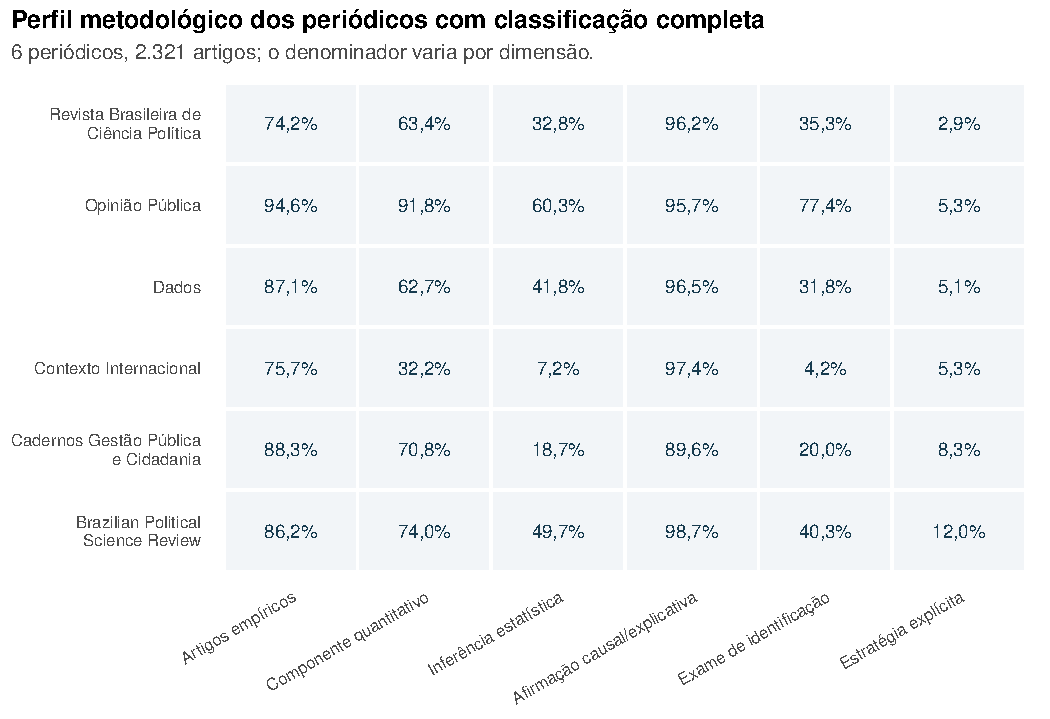
\includegraphics[width=0.95\linewidth]{../output/figures/paper/figure_2_journal_dimension_matrix} \caption{As práticas metodológicas variam entre os seis periódicos integralmente classificados. Empíricos e examinados usam todos os artigos; análise quantitativa usa os empíricos; inferência estatística usa os quantitativos com rótulo observado; estratégia explícita usa os examinados.}\label{fig:figura-2}
\end{figure}

A diferença mais nítida está na inferência estatística entre artigos
quantitativos: 60,3\% em \texttt{Opinião\ Pública}, 49,7\% na BPSR e
41,8\% em \texttt{Dados}, contra 18,7\% em CGPC e 7,2\% em
\texttt{Contexto\ Internacional}. Esses contrastes podem refletir
diferenças de composição temática, tradição disciplinar e política
editorial que o desenho atual não permite decompor; não constituem
ranking de qualidade nem efeito causal do periódico.

O perfil agregado de CGPC cobre apenas 2019--2025, enquanto os demais
periódicos completos contribuem também em períodos anteriores. Sua
comparação histórica direta com os outros cinco, portanto, combina
diferenças editoriais e composição temporal.

\subsection{Inferência estatística}\label{inferuxeancia-estatuxedstica}

Na cobertura classificada, 618 de 1.629 artigos quantitativos com rótulo
observado apresentam inferência estatística (37,9\%). A comparação mais
segura usa os seis periódicos completos: são 551 de 1.281, ou 43,0\%.
Apenas \texttt{Opinião\ Pública} ultrapassa 50\%; BPSR fica em 49,7\%, e
os outros quatro periódicos ficam abaixo desse patamar.

A taxa agregada baixa reflete principalmente o tipo de análise
quantitativa publicada. Entre os casos com rótulo observado, 634 de
1.281 artigos foram classificados como estatística descritiva e sem
inferência (49,5\%). Outros 9 combinam o rótulo de categoria descritiva
com inferência positiva e exigem adjudicação. Entre os 638 trabalhos com
rótulo observado que usam testes bivariados, correlações ou modelagem
estatística, 542 apresentam alguma quantificação formal de incerteza
(85,0\%); 3 dos 641 trabalhos dessas categorias não têm rótulo de
inferência. O estrato analisado, portanto, não se caracteriza sobretudo
por modelos publicados sem erros-padrão ou intervalos, mas por uma
produção quantitativa em grande medida descritiva.

No suporte temporal comum, as proporções observadas não sugerem
crescimento da inferência: passam de 46,1\% em 2005--2011 para 44,2\% em
2012--2018 e 44,1\% em 2019--2025. Essa estabilidade é exploratória
porque período e configuração do classificador não estão completamente
separados.

A Figura 3 oferece um benchmark internacional com três periódicos
generalistas canônicos: APSR, AJPS e \emph{Journal of Politics}.
Torreblanca et al. (\citeproc{ref-torreblanca2026}{2026}) encontram
abordagens baseadas em desenho causal em 45,4\% dos artigos
quantitativos explicativos do \emph{Journal of Politics}, 47,0\% da AJPS
e 56,8\% da APSR. A média ponderada dos percentuais e denominadores
tabulados é 48,4\%. Esses números ficam próximos dos 43,0\% brasileiros,
mas a coincidência de magnitudes serve apenas para colocar o resultado
em perspectiva. As medidas variam no atributo classificado, no
denominador, na composição editorial e no período. A seleção
internacional de artigos explicativos torna o denominador mais orientado
a métodos, enquanto seu numerador é mais restritivo. A justaposição não
estima um hiato internacional nem permite comparar diretamente
prevalência ou credibilidade.

\begin{figure}
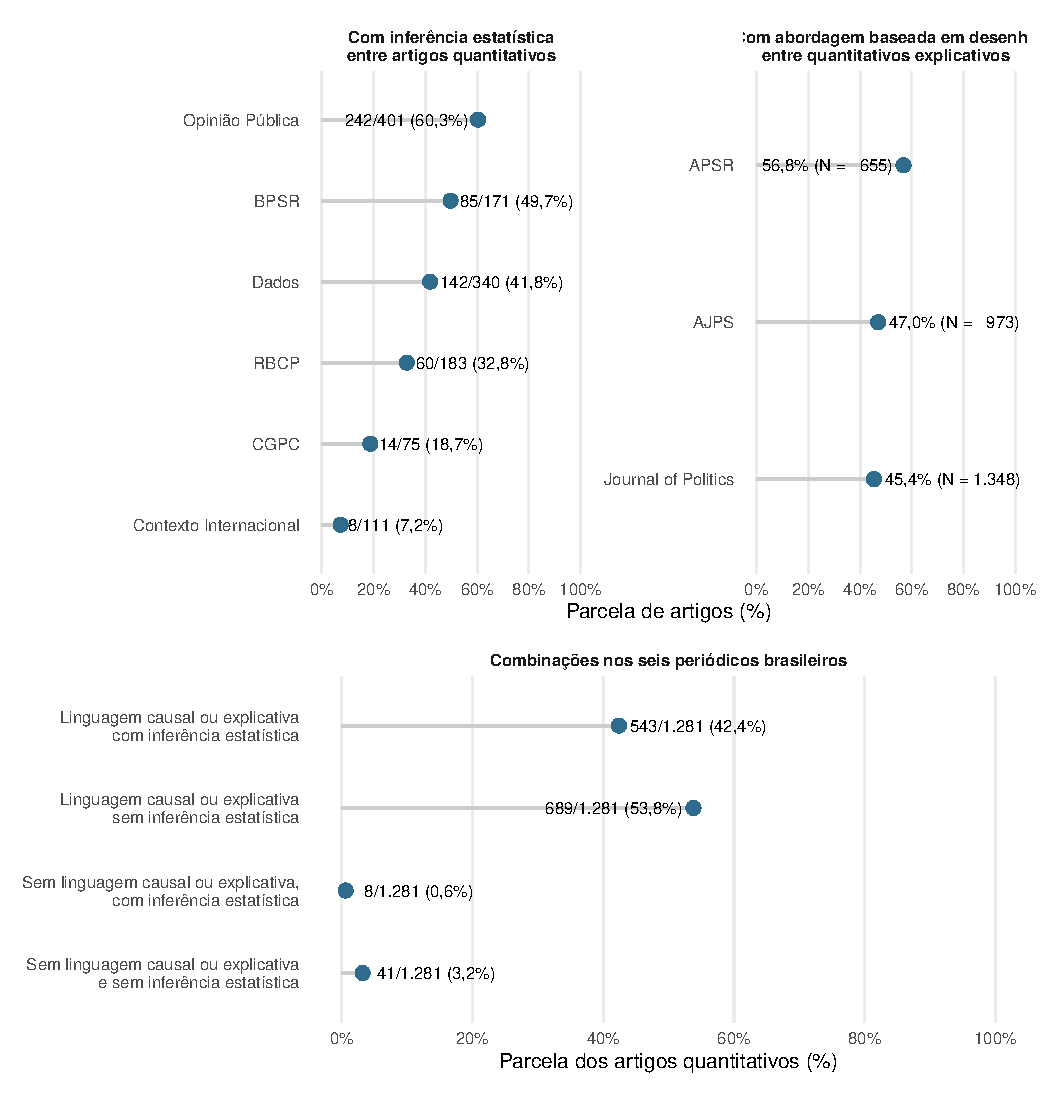
\includegraphics[width=0.95\linewidth]{../output/figures/paper/figure_statistical_inference_benchmark} \caption{Práticas distintas têm magnitudes numericamente próximas, mas não diretamente comparáveis. À esquerda, parcela com quantificação formal da incerteza entre os artigos quantitativos dos seis periódicos brasileiros, de 2005 a 2025; os rótulos apresentam numerador/denominador. À direita, parcela com abordagem baseada em desenho causal entre os artigos quantitativos explicativos da APSR, AJPS e Journal of Politics, de 2003 a 2023; N é o denominador, conforme a tabela suplementar de Torreblanca et al. As medidas e os universos diferem; a justaposição situa ordens de grandeza e não estima um hiato internacional.}\label{fig:figura-inferencia-benchmark}
\end{figure}

\subsection{Evidência qualitativa}\label{eviduxeancia-qualitativa}

Nos seis periódicos completos, 1.352 artigos apresentam evidência
qualitativa, isoladamente ou em combinação com evidência quantitativa. O
classificador identifica objetivo qualitativo claro em 1.261 deles, ou
93,3\%. Esse resultado indica que o propósito substantivo da análise
qualitativa costuma ser reconstruível, mas não mede explicitação de
seleção de casos, procedimentos interpretativos ou rastreabilidade
documental. Portanto, não substitui a futura variável de explicitação
metodológica.

\subsection{Linguagem causal ou explicativa ampla e estratégias de
identificação}\label{linguagem-causal-ou-explicativa-ampla-e-estratuxe9gias-de-identificauxe7uxe3o}

A categoria de linguagem causal ou explicativa é deliberadamente ampla.
Ela aparece em 3.194 artigos, dos quais 2.726 são empíricos. A Figura 4
é um diagnóstico dessa amplitude e mostra por que a variável não
discrimina pretensões causais estritas: há marcações em artigos não
empíricos, em artigos empíricos sem componente quantitativo e em artigos
empíricos quantitativos sem estratégia explícita de identificação. Esses
cruzamentos descrevem coexistência de atributos; não medem
desalinhamento ou adequação entre afirmação e método.

\begin{figure}
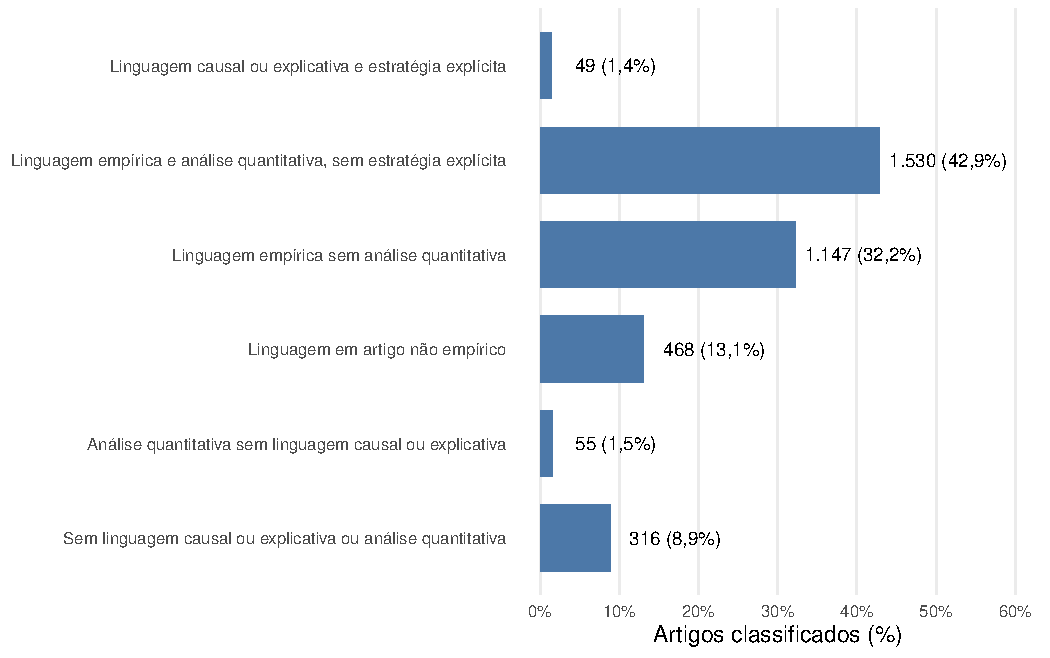
\includegraphics[width=0.95\linewidth]{../output/figures/paper/figure_5_claim_method_alignment} \caption{Combinações entre linguagem causal ou explicativa, análise quantitativa e estratégias explícitas nos 3.565 artigos classificados. As categorias são mutuamente exclusivas; os rótulos mostram número e percentual de artigos.}\label{fig:figura-5}
\end{figure}

No conjunto parcial dos artigos classificados, 49 dos 1.116 selecionados
pelo protocolo para examinar identificação mencionam ao menos uma
estratégia explícita, equivalentes a 4,4\%. No estrato principal dos
seis periódicos completos, a proporção é 49 em 846, ou 5,8\%. Como esse
subconjunto inclui afirmações explicativas amplas e modelagem
quantitativa, ele não contém apenas estudos causais. A Tabela 4 mantém
visíveis os diferentes denominadores. As categorias diagnósticas não são
mutuamente exclusivas e não devem ser somadas como uma distribuição.

\begin{longtable}[]{@{}
  >{\raggedright\arraybackslash}p{(\linewidth - 6\tabcolsep) * \real{0.5368}}
  >{\raggedright\arraybackslash}p{(\linewidth - 6\tabcolsep) * \real{0.0632}}
  >{\raggedright\arraybackslash}p{(\linewidth - 6\tabcolsep) * \real{0.2842}}
  >{\raggedright\arraybackslash}p{(\linewidth - 6\tabcolsep) * \real{0.1158}}@{}}
\caption{Linguagem causal ou explicativa e estratégias explícitas de
identificação.}\tabularnewline
\toprule\noalign{}
\begin{minipage}[b]{\linewidth}\raggedright
Categoria
\end{minipage} & \begin{minipage}[b]{\linewidth}\raggedright
N
\end{minipage} & \begin{minipage}[b]{\linewidth}\raggedright
Denominador
\end{minipage} & \begin{minipage}[b]{\linewidth}\raggedright
Percentual
\end{minipage} \\
\midrule\noalign{}
\endfirsthead
\toprule\noalign{}
\begin{minipage}[b]{\linewidth}\raggedright
Categoria
\end{minipage} & \begin{minipage}[b]{\linewidth}\raggedright
N
\end{minipage} & \begin{minipage}[b]{\linewidth}\raggedright
Denominador
\end{minipage} & \begin{minipage}[b]{\linewidth}\raggedright
Percentual
\end{minipage} \\
\midrule\noalign{}
\endhead
\bottomrule\noalign{}
\endlastfoot
Linguagem causal ou explicativa & 3.194 & Todos (3.565) & 89,6\% \\
Linguagem causal ou explicativa em artigo empírico & 2.726 & Empíricos
(2.825) & 96,5\% \\
Artigos examinados & 1.116 & Todos (3.565) & 31,3\% \\
Estratégia explícita & 49 & Artigos examinados (1.116) & 4,4\% \\
Sem estratégia explícita & 1.066 & Artigos examinados (1.116) &
95,5\% \\
Outras estratégias codificadas & 9 & Artigos examinados (1.116) &
0,8\% \\
\end{longtable}

Nos seis periódicos completos, 49 dos 846 artigos examinados mencionam
ao menos uma estratégia explícita de identificação causal.
Diferenças-em-diferenças, pareamento ou ponderação, experimentos em
survey e regressão descontínua são as famílias mais frequentes. A Figura
5 conta ocorrências artigo-método; um mesmo artigo pode mobilizar mais
de uma estratégia. A contagem não audita a execução nem a plausibilidade
dos pressupostos.

\begin{figure}[H]
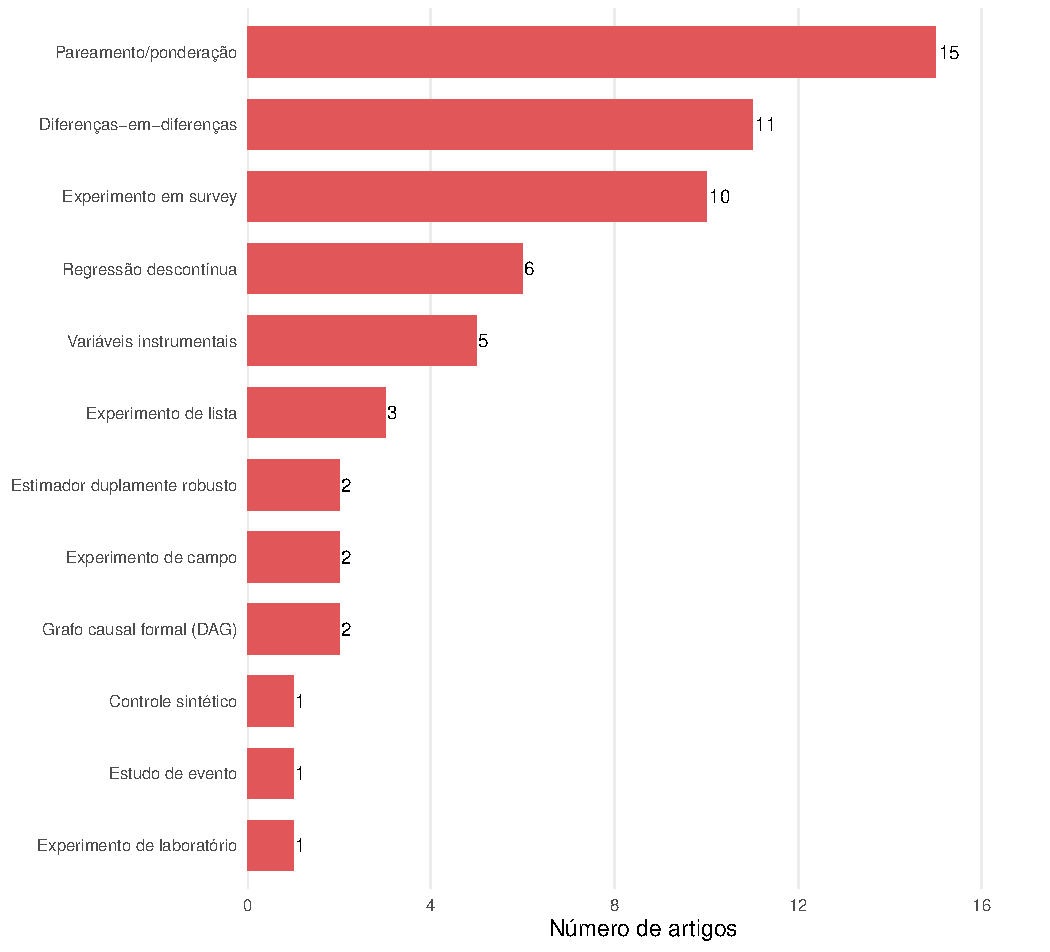
\includegraphics[width=0.95\linewidth]{../output/figures/paper/figure_6_strict_method_distribution} \caption{Estratégias explícitas de identificação nos seis periódicos integralmente classificados. As barras contam os artigos que mencionam cada estratégia; um artigo pode mencionar mais de uma.}\label{fig:figura-6}
\end{figure}

\subsection{Variação por período}\label{variauxe7uxe3o-por-peruxedodo}

A comparação temporal usa BPSR, \texttt{Contexto\ Internacional},
\texttt{Dados}, \texttt{Opinião\ Pública} e RBCP, os cinco periódicos
completos presentes nos três períodos agregados. A presença média de
artigos empíricos cresce de 71,5\% em 2005--2011 para 88,3\% em
2019--2025. Para quantificação, a conclusão depende da ponderação: com
peso igual por periódico, a proporção passa de 56,2\% para 66,5\%;
agrupando os artigos, passa de 65,1\% para 67,5\%, com queda
intermediária. O aumento equiponderado é concentrado sobretudo na RBCP,
que parte de apenas 2 artigos quantitativos entre 12 empíricos em
2005--2011 (16,7\%) e alcança 71,1\% em 2019--2025. Para inferência
estatística, a média equiponderada cresce de 29,9\% para 39,4\%,
enquanto a proporção agrupada passa de 46,1\% para 44,1\%. O resultado
mais prudente é crescimento da empiria, estabilidade aproximada da
quantificação e da inferência quando os artigos são agrupados, e forte
sensibilidade das médias equiponderadas à composição dos periódicos.
Estratégias explícitas de identificação continuam raras e não apresentam
trajetória monotônica.

\begin{longtable}[]{@{}
  >{\raggedright\arraybackslash}p{(\linewidth - 8\tabcolsep) * \real{0.2706}}
  >{\raggedright\arraybackslash}p{(\linewidth - 8\tabcolsep) * \real{0.3765}}
  >{\raggedright\arraybackslash}p{(\linewidth - 8\tabcolsep) * \real{0.1176}}
  >{\raggedright\arraybackslash}p{(\linewidth - 8\tabcolsep) * \real{0.1176}}
  >{\raggedright\arraybackslash}p{(\linewidth - 8\tabcolsep) * \real{0.1176}}@{}}
\caption{Quantificação e inferência estatística por período, segundo a
regra de ponderação.}\tabularnewline
\toprule\noalign{}
\begin{minipage}[b]{\linewidth}\raggedright
Dimensão
\end{minipage} & \begin{minipage}[b]{\linewidth}\raggedright
Ponderação
\end{minipage} & \begin{minipage}[b]{\linewidth}\raggedright
2005-2011
\end{minipage} & \begin{minipage}[b]{\linewidth}\raggedright
2012-2018
\end{minipage} & \begin{minipage}[b]{\linewidth}\raggedright
2019-2025
\end{minipage} \\
\midrule\noalign{}
\endfirsthead
\toprule\noalign{}
\begin{minipage}[b]{\linewidth}\raggedright
Dimensão
\end{minipage} & \begin{minipage}[b]{\linewidth}\raggedright
Ponderação
\end{minipage} & \begin{minipage}[b]{\linewidth}\raggedright
2005-2011
\end{minipage} & \begin{minipage}[b]{\linewidth}\raggedright
2012-2018
\end{minipage} & \begin{minipage}[b]{\linewidth}\raggedright
2019-2025
\end{minipage} \\
\midrule\noalign{}
\endhead
\bottomrule\noalign{}
\endlastfoot
Quantificação & Peso igual por periódico & 56,2\% & 63,8\% & 66,5\% \\
Quantificação & Artigos agrupados & 65,1\% & 63,4\% & 67,5\% \\
Inferência estatística & Peso igual por periódico & 29,9\% & 38,4\% &
39,4\% \\
Inferência estatística & Artigos quantitativos agrupados & 46,1\% &
44,2\% & 44,1\% \\
\end{longtable}

\begin{figure}
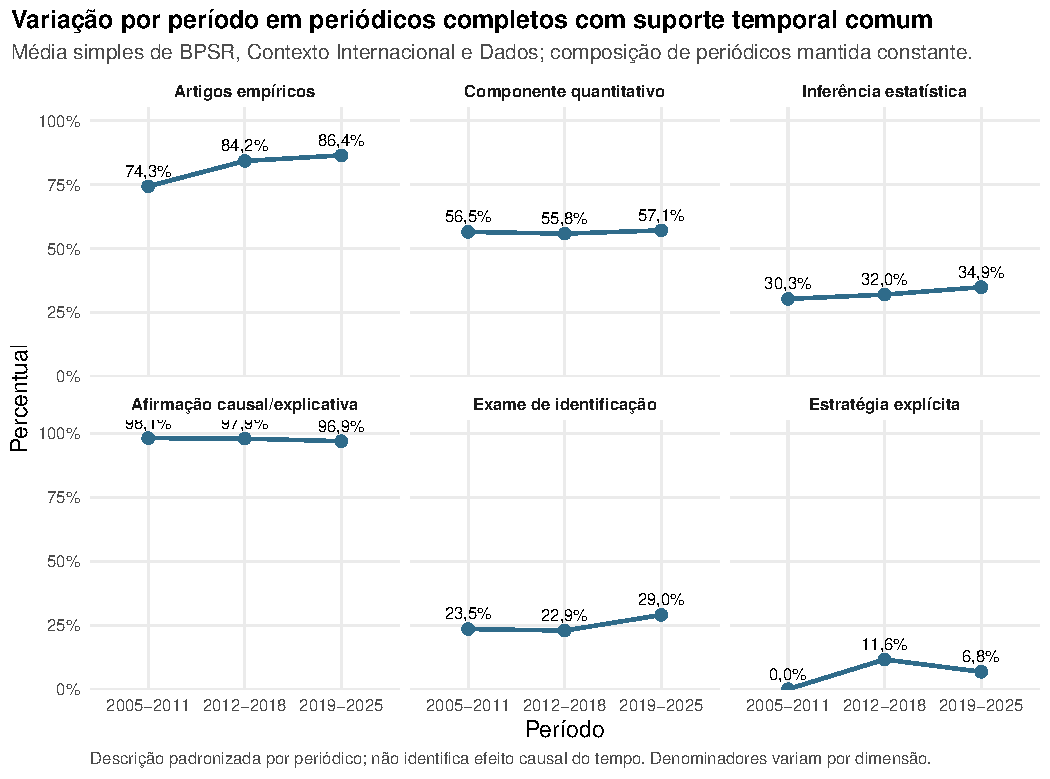
\includegraphics[width=0.95\linewidth]{../output/figures/paper/figure_3_period_variation} \caption{A presença de artigos empíricos cresce entre os períodos, enquanto estratégias explícitas permanecem raras. Os pontos são médias com peso igual para BPSR, Contexto Internacional, Dados, Opinião Pública e RBCP; todos os painéis usam escala de 0\% a 100\%.}\label{fig:figura-3}
\end{figure}

\newpage

\section{Discussão}\label{discussuxe3o}

O principal achado é a distância entre quantificação e inferência
estatística. Nos seis periódicos completos, apenas 43,0\% dos artigos
quantitativos apresentam teste, intervalo ou procedimento equivalente de
quantificação da incerteza. Essa frequência não cresce no suporte
temporal comum: permanece entre 44,1\% e 46,1\% nos três períodos. A
expansão da pesquisa empírica, portanto, não foi acompanhada por difusão
semelhante da inferência formal.

A decomposição qualifica esse diagnóstico. 49,5\% dos artigos
quantitativos com rótulo observado foram classificados como descritivos
e sem inferência, enquanto 85,0\% dos trabalhos com testes bivariados ou
modelagem e rótulo observado apresentam inferência. Nove conflitos entre
categoria descritiva e inferência positiva permanecem para adjudicação.
O gargalo agregado parece residir mais na composição da produção
quantitativa do que na omissão generalizada de incerteza em análises
formalmente modeladas. Isso mede incidência, não necessidade: uma
análise descritiva pode responder adequadamente a uma pergunta
descritiva sem recorrer a testes ou intervalos. Ainda assim, registrar
um valor de \emph{p}, erro-padrão ou intervalo não garante validade:
esta análise não avalia poder, especificação, multiplicidade,
calibração, dependência dos dados ou interpretação substantiva.

A comparação com Torreblanca et al.~coloca a magnitude em perspectiva,
mas não testa nem reforça uma explicação para o resultado brasileiro. A
taxa de inferência formal (43,0\%) fica 5,4\% abaixo da média ponderada
dos percentuais tabulados de desenhos causais em APSR, AJPS e
\emph{Journal of Politics}. O atributo, o denominador, a composição
editorial e o período diferem entre os estudos. A proximidade é digna de
nota justamente porque desenhos causais constituem um padrão mais
restritivo, mas não representa comparação equivalente de desempenho.

Os seis periódicos completos também mostram que a prática metodológica
não se organiza em uma única escala. \texttt{Opinião\ Pública}, BPSR e
\texttt{Dados} combinam elevada presença empírica com maior frequência
de inferência; \texttt{Contexto\ Internacional} é amplamente empírico,
mas sobretudo qualitativo e pouco orientado à inferência estatística;
CGPC combina elevada empiria e quantificação com menor frequência de
inferência. A RBCP ocupa posição intermediária. Essas diferenças são
descritivas e podem refletir composição temática, áreas, tipos de
pergunta e políticas editoriais; o desenho não separa essas explicações.

A análise temporal reforça essa multidimensionalidade. Nos cinco
periódicos presentes nos três períodos agregados, a proporção de artigos
empíricos cresce. Quantificação e inferência aumentam na média que dá
peso igual aos periódicos, mas permanecem aproximadamente estáveis
quando os artigos são agrupados; o aumento equiponderado da
quantificação é fortemente influenciado pela RBCP. Não há difusão
monotônica das famílias de desenho. Os resultados preliminares não
sustentam uma narrativa de marcha uniforme rumo à quantificação, à
inferência estatística ou a desenhos causais.

A categoria ampla de afirmação causal ou explicativa precisa ser
interpretada com especial cautela. Sua frequência elevada não significa
que quase todos os artigos façam inferência causal: ela também registra
explicações qualitativas, argumentos teóricos e interpretações
substantivas. O subconjunto de 1.116 artigos selecionado para examinar
identificação não contém apenas estudos causais, e os 49 casos positivos
registram famílias de método mencionadas no texto. A diferença entre
essas contagens é uma descrição taxonômica útil, mas não mede
diretamente credibilidade, adequação entre afirmação e método ou
qualidade da identificação. Além disso, os 270 casos examinados nos
periódicos parciais contêm 0 positivos, enquanto os 846 casos dos
periódicos completos contêm todos os 49 positivos. Essa concentração
pode refletir diferenças substantivas entre periódicos, mas também a
configuração dos lotes; por isso, o agregado parcial não sustenta
comparação editorial e exige reclassificação de validação com
configuração comum.

O pluralismo metodológico delimita a interpretação dos resultados. A
ausência de uma estratégia explícita de identificação causal não
representa deficiência em todo tipo de artigo, e sua presença nominal
não demonstra qualidade. Esta versão mapeia a incidência de práticas
empíricas, quantitativas, inferenciais e de identificação; não mede a
adequação entre cada afirmação e o método empregado.

\section{Conclusão}\label{conclusuxe3o}

Nos seis periódicos integralmente classificados, a presença elevada de
artigos empíricos convive com baixa incidência agregada de inferência
estatística: 551 de 1.281 artigos quantitativos (43,0\%). A taxa
permanece próxima de 44\% nos três períodos do suporte comum. Embora
85,0\% dos artigos com testes bivariados ou modelagem e rótulo observado
quantifiquem incerteza, 49,5\% dos quantitativos observados são
classificados como descritivos e sem inferência. O avanço da empiria não
se traduziu em difusão equivalente da inferência formal.

A proximidade entre essa taxa e a parcela de desenhos causais nos três
periódicos internacionais de referência é um benchmark descritivo, não
uma equivalência. O resultado brasileiro mede uma prática mais básica em
um conjunto mais amplo de artigos quantitativos; o resultado de
Torreblanca et al.~mede identificação causal entre artigos quantitativos
explicativos. Os números colocam a baixa incidência brasileira em
perspectiva, mas não permitem uma comparação direta de prevalência ou
credibilidade.

Nos seis periódicos integralmente classificados, apenas 49 dos 846
artigos selecionados pelo protocolo para examinar identificação
mencionam uma estratégia explícita, equivalentes a 5,8\%. No conjunto
parcial de 3.565 artigos, a referência correspondente é 49 em 1.116, ou
4,4\%. Essas frequências descrevem presença nominal, não qualidade
metodológica. Como a classificação automatizada ainda requer validação
humana e cobre apenas parte do universo de 5.249 artigos, as comparações
editoriais permanecem restritas aos seis periódicos integralmente
classificados.

\newpage

\appendix

\section{Apêndice: Cobertura e variação
anual}\label{apuxeandice-cobertura-e-variauxe7uxe3o-anual}

A Figura 7 detalha a cobertura da classificação por periódico. Seis
periódicos estão completos e cinco estão parcialmente classificados;
todos os onze já têm artigos classificados. A distribuição ainda
desigual impede transformar a média dos 3.565 casos em estimativa da
produção brasileira como um todo.

\begin{figure}
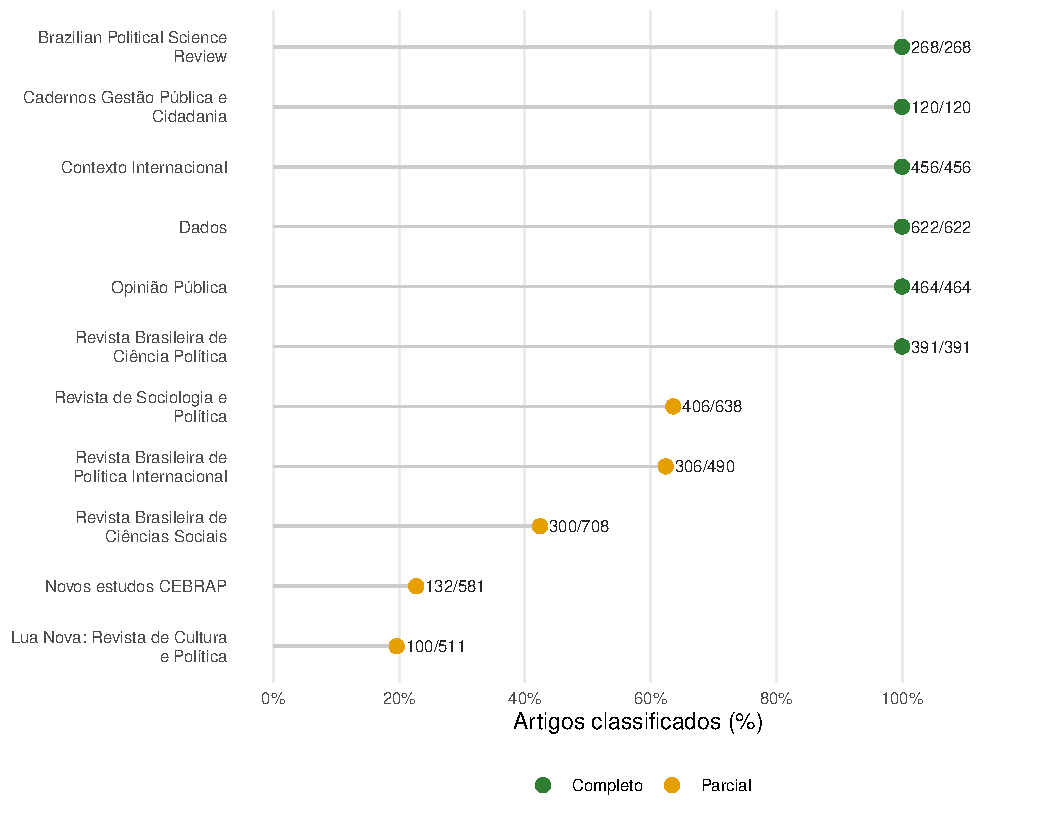
\includegraphics[width=0.95\linewidth]{../output/figures/paper/figure_4_journal_period_coverage} \caption{Seis dos onze periódicos estão integralmente classificados. Os pontos mostram a proporção classificada, e os rótulos, artigos classificados/elegíveis.}\label{fig:figura-4}
\end{figure}

A Figura 8 apresenta as mesmas dimensões por ano para revelar variações
que os três períodos agregados podem ocultar. Para manter a composição
dos periódicos, ela inclui apenas 2011--2025, intervalo em que BPSR,
\texttt{Contexto\ Internacional}, \texttt{Dados},
\texttt{Opinião\ Pública} e RBCP têm artigos em todos os anos. As
proporções anuais agrupam os artigos dos cinco periódicos, enquanto a
Figura 6 dá peso igual a cada periódico; por isso, os níveis das duas
figuras não devem ser comparados diretamente. As oscilações anuais são
descritivas e podem refletir denominadores pequenos.

\begin{figure}
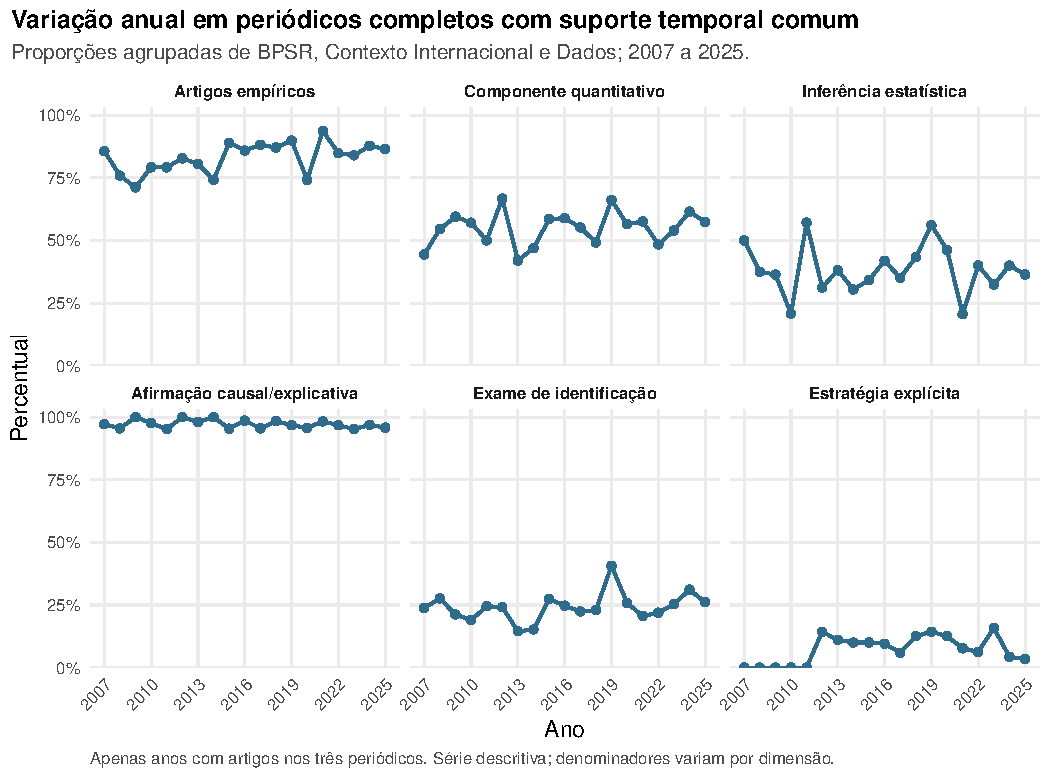
\includegraphics[width=0.95\linewidth]{../output/figures/paper/figure_7_year_variation} \caption{As séries anuais mostram crescimento da empiria e oscilação das demais práticas entre 2011 e 2025. As proporções agrupam os artigos de BPSR, Contexto Internacional, Dados, Opinião Pública e RBCP e incluem apenas anos com publicação nos cinco periódicos; todos os painéis usam escala de 0\% a 100\%.}\label{fig:figura-7}
\end{figure}

\clearpage

\small

\section*{Referências}\label{referuxeancias}
\addcontentsline{toc}{section}{Referências}

\protect\phantomsection\label{refs}
\begin{CSLReferences}{1}{0}
\bibitem[\citeproctext]{ref-albuquerque2022}
Albuquerque, Rodrigo Barros de, Rafael Mesquita, and Renato Victor Lira
Brito. 2022. {``{Obscuridade metodológica: um mapeamento da formação em
métodos na pós-graduação em Relações Internacionais e áreas afins no
Brasil}.''} \emph{Revista Brasileira de Ciência Política}, no. 39.
\url{https://doi.org/10.1590/0103-3352.2022.39.258379}.

\bibitem[\citeproctext]{ref-barberia2014}
Barberia, Lorena Guadalupe, Samuel Ralize de Godoy, and Danilo Praxedes
Barboza. 2014. {``{Novas perspectivas sobre o calcanhar metodológico: o
ensino de métodos de pesquisa em Ciência Política no Brasil}.''}
\emph{Teoria \& Sociedade} 22 (2).

\bibitem[\citeproctext]{ref-figueiredo2019}
Figueiredo Filho, Dalson Britto, Rodrigo Lins, Amanda Domingos, Nicole
Janz, and Lucas Silva. 2019. {``Seven Reasons Why: A User's Guide to
Transparency and Reproducibility.''} \emph{Brazilian Political Science
Review} 13 (2). \url{https://doi.org/10.1590/1981-3821201900020001}.

\bibitem[\citeproctext]{ref-soares2005}
Soares, Gláucio Ary Dillon. 2005. {``{O calcanhar metodológico da
ciência política no Brasil}.''} \emph{Sociologia, Problemas e Práticas},
no. 48: 27--52.

\bibitem[\citeproctext]{ref-torreblanca2026}
Torreblanca, Carolina, William Dinneen, Guy Grossman, and Yiqing Xu.
2026. {``The Credibility Revolution in Political Science.''}
arXiv:2601.11542. \url{https://arxiv.org/abs/2601.11542}.

\end{CSLReferences}

\end{document}
